\documentclass[final,t]{beamer}
\mode<presentation>
{
%\usetheme{Lankton}
%  \usetheme{Berlin} 
%  \usetheme{Warsaw}
%  \usetheme{Aachen}
%  \usetheme{Oldi6}
%  \usetheme{I6td}
%  \usetheme{I6dv}
%  \usetheme{I6pd}
%  \usetheme{I6pd2}
%  \usetheme{PHI6}
%  \usetheme{PHCVD}
  \usetheme{PH}
%\usetheme{Icy2}
}

% additional settings
\setbeamerfont{itemize}{size=\normalsize}
\setbeamerfont{itemize/enumerate body}{size=\normalsize}
\setbeamerfont{itemize/enumerate subbody}{size=\normalsize}

%additional packages
%\usepackage{times} 
\usepackage{amsmath,amsthm, amssymb, latexsym}
\usepackage{exscale} 
\usepackage{booktabs, array}
\usepackage{rotating} %sideways environment 
\usepackage[english]{babel}
%\usepackage[latin1]{inputenc}
\usefonttheme{professionalfonts}
%\usefonttheme{serif} % default family is serif
%\usepackage{euler}
\usepackage{fontspec}
%\setmainfont{Liberation Serif}
\usepackage{xspace}
\usepackage{url}
\usepackage{hyperref}
\usepackage{multicol}
\usepackage{xspace}
%\usepackage{natbib}
\usepackage{booktabs}
\usepackage{dcolumn}
\newcommand{\Lagr}{\mathcal{L}}
\usepackage{multicol}
\usepackage[authordate,numbermonth=false,doi=false,isbn=false,backend=biber]{biblatex-chicago}
\DeclareFieldFormat[article,inbook,incollection,inproceedings,patent,thesis,unpublished]{title}{\mkbibquote{#1\isdot}}
%\addbibresource{MLE.bib}
\nocite{*}
\usepackage[orientation=landscape,size=a0,scale=1]{beamerposter}
%\usepackage{Sweave}
\usepackage{ragged2e}
%\apptocmd{\frame}{\justifying}{}{}

\setbeamercolor{enumerate item}{ fg=Plum}
\setbeamercolor{itemize item}{ fg=Plum}
\setbeamertemplate{bibliography item}{}

%\usecaptiontemplate{\small\structure{\insertcaptionname~\insertcaptionnumber: }\insertcaption}% 
\setbeamertemplate{caption}[numbered]
\setbeamercolor{caption name}{fg=Plum}

% To produce both postscript and pdf graphics, remove the eps and pdf
% parameters in the next line. Set default plot size to 5 x 3.5 in.

%\listfiles
%\graphicspath{{figures/}}
% Display a grid to help align images
%\beamertemplategridbackground[1cm]

\title{POSTER!}
\author[Sarah B. Bouchat]{Sarah B. Bouchat}
\institute[University of Wisconsin--Madison]{University of Wisconsin--Madison}
\date[24 Sept 2014]{24 September 2014}

%\DefineVerbatimEnvironment{Sinput}{Verbatim} {xleftmargin=2em}
%\DefineVerbatimEnvironment{Soutput}{Verbatim}{xleftmargin=2em}
%\DefineVerbatimEnvironment{Scode}{Verbatim}{xleftmargin=2em}
%\fvset{listparameters={\setlength{\topsep}{0pt}}}
%\renewenvironment{Schunk}{\vspace{\topsep}}{\vspace{\topsep}}


\makeatletter
\DeclareRobustCommand\onedot{\futurelet\@let@token\@onedot}
\def\@onedot{\ifx\@let@token.\else.\null\fi\xspace}
\def\eg{{e.g}\onedot} \def\Eg{{E.g}\onedot}
\def\ie{{i.e}\onedot} \def\Ie{{I.e}\onedot}
\def\cf{{c.f}\onedot} \def\Cf{{C.f}\onedot}
\def\etc{{etc}\onedot}
\def\vs{{vs}\onedot}
\def\wrt{w.r.t\onedot}
\def\dof{d.o.f\onedot}
\def\etal{{et al}\onedot}
\makeatother

%%%%%%%%%%%%%%%%%%%%%%%%%%%%%%%%%%%%%%%%%%%%%%%%%%%%%%%%%%%%%%%%%%%%%%%%%%%%%%%%%%%%%%%%%%%%%%%%%%%%%%%%%%%%
\setbeamercolor{background canvas}{bg=Apricot}
\begin{document}
\colorlet{i6colorscheme3}{Apricot}
\addtobeamertemplate{block end}{}{\vspace*{2ex}}
%\input{beamerpostertest-concordance}
%\bibliographystyle{plainnat}

\begin{frame}[fragile]
  \begin{columns}[t]

    %-- Column 1 ---------------------------------------------------
    \begin{column}{0.32\linewidth}

      %-- Block 1-1
      \begin{block}{Summary \& Motivation}
       This is a poster containing text and other things, notably attractive visual displays...
        This part is the summary of the paper you picked, what they did, and what's wrong with it.  People might read this.
      \end{block}

%-- Block 1-5
      \begin{block}{Replication}
     For example, in this block, I've put some pretty pictures!
\begin{figure}[htb]
        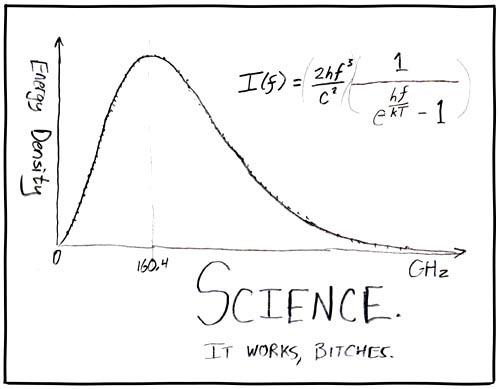
\includegraphics[height=5.75in, width=.45\columnwidth]{science.png}
            \caption{Some basic models perhaps} 
        \end{figure}
\end{block}

\begin{block}{FYI regarding columns}
The columns will automatically align with each other and try to look
        as nice as possible.  You may have to add {\tt$\backslash$vspace\{1pt\}}
        commands to adjust the spacing here and there.  Remember that you can
        use positive or negative numbers.
        \end{block}
    \end{column}%1

    %-- Column 2 ---------------------------------------------------
    \begin{column}{0.32\linewidth}

     %-- Block 2-1
      \begin{block}{Lists}
      Just as with regular \LaTeX and beamer...
      \begin{itemize}
          \item You can make
          \item lists, that
          \item allow people to see what you concluded
          \item quickly
        \end{itemize}
      \end{block}

%-- Block 2-2
      \begin{block}{Math}
        Include math within the text is as simple as $1+1=2$.  You can also
        highlight more important equations like this:
        \begin{equation*}
          \int_0^1\sin(x)+\cos^2(x)+\alpha x~d\!x
        \end{equation*}
  \vspace{10pt}

      \begin{equation*}
          P(Y=y) = \left\{ \begin{array}{l l} p+ (1-p)(1+\frac{\lambda}{\tau})^{-\tau}, & \quad y=0 \\
          \vspace{10pt}
	(1-p)\frac{\Gamma(y+\tau)}{y!\Gamma (\tau)}(1+ \frac{\lambda}{\tau})^{-\tau}(1+\frac{\tau}{\lambda})^{-y}, &  \quad y=1, 2, ..., n 
	\end{array} \right.
        \end{equation*}
        \end{block}
        
    \end{column}%2

    %-- Column 3 ---------------------------------------------------
    \begin{column}{0.32\linewidth}

%-- Block 2-4
      \begin{block}{Results}   
      \begin{multicols}{2}
      \vspace{-30pt}
        \begin{figure}[htb]
        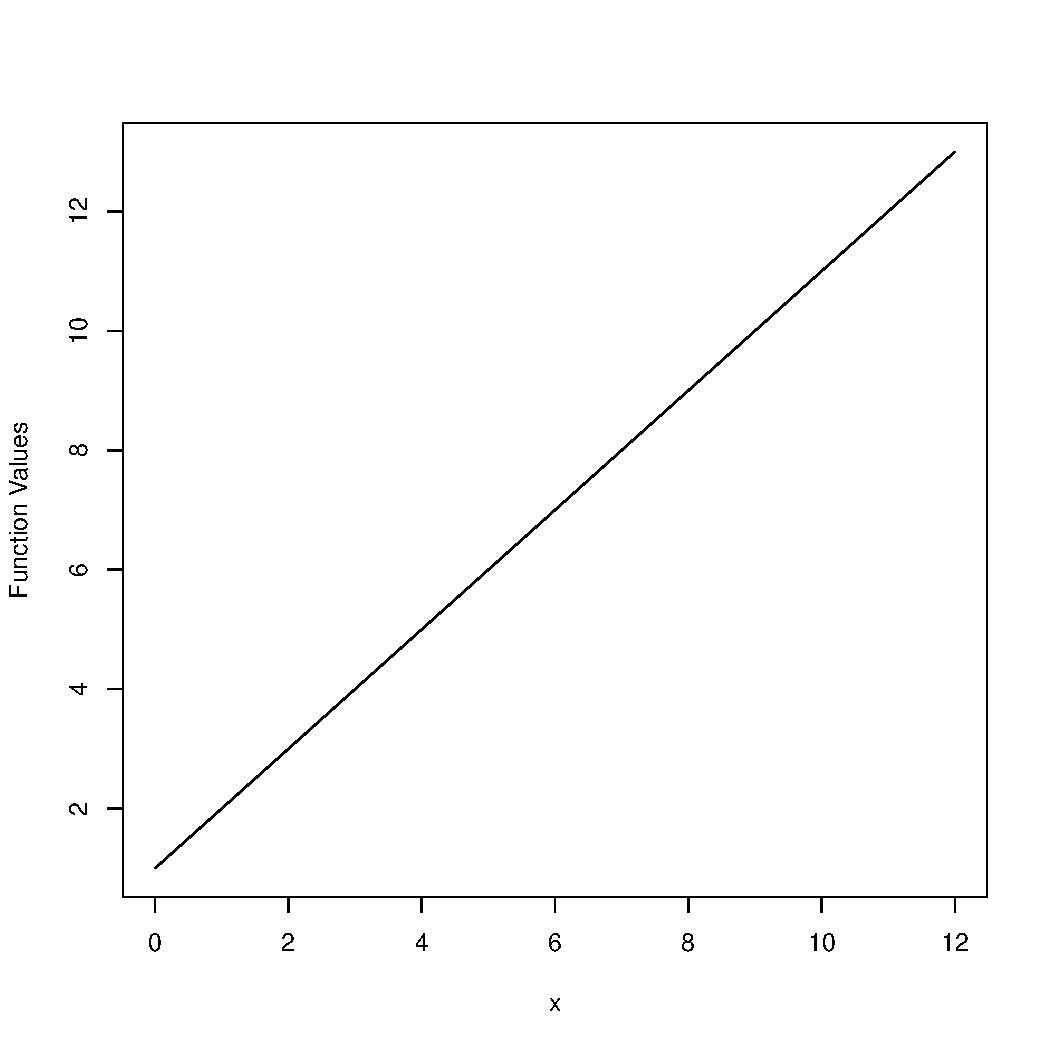
\includegraphics[height=7.5in, width=1.05\columnwidth]{myprettypicture.pdf}
         \caption{This picture is very pretty, don't you think?}
        \end{figure}
              Here you'll present graphical results with explanation, probably. \\
              \vspace{15pt}
              You might want to do things this way if you have contrasting results you want to present side-by-side, for example.
        \end{multicols}
      \end{block}


      %-- Block 3-3
       
%\begin{block}{Predicted Outcomes: Negative Binomial vs. Zero-Inflated}
  %  \end{block}
    
    \begin{block}{Conclusions}
        What did you conclude? What additional work needs to be done?
        \vspace{20pt}
\begin{itemize}
  \item I did something great, get excited.
  \vspace{10pt}
  \item More work for us!
\end{itemize}
      \end{block}
%-- Block 3-4
      \begin{block}{References}
			% Note: Rsystem reference is defined inside feh.bib. It is a slightly
			% edited version of the output of citation().
			Just as with regular \LaTeX documents, you can include a \verb+.bib+ file in the folder, and cite references on your poster
			\scriptsize
			\printbibliography[heading=none]
			%\bibliography{testwhyR}
			\normalsize
		\end{block}
 
% \begin{block}{Creative Commons Sharealike}
 %\includegraphics[width=.15\columnwidth]{cc_attribution_sharealike}
 %\end{block}
 
    \end{column}%3

  \end{columns}

\end{frame}


\end{document}


      %-- Block 3-1
      \begin{block}{Experiments}
        Remember to put lots of figures on your poster... Nobody reads anymore!
        \\
        {\tiny tiny size}\\
        {\scriptsize scriptsize size}\\
        {\footnotesize footnotesize size}\\
        {\small small size}\\
        {\normalsize normalsize size}\\
        {\large large size}\\
        {\Large Large size}\\
        {\LARGE LARGE size}\\
        {\huge huge size}\\
        {\Huge Huge size}\\
        
      \end{block}



  %-- Block 3-2
      \begin{alertblock}{Conclusion}
        This is an alert block.  Much less annoying than PowerPoint.  Copy and Paste from your
        document. Overall, a great idea!
      \end{alertblock}

%-- Block 1-4
\begin{block}{Tables}
You can insert tables of data
\begin{tabular}{rrlr}
  \hline
x & y & type & z \\ 
  \hline
  1 & 44.60 & Red & 46.07 \\ 
    2 & 61.32 & Blue & 63.60 \\ 
    3 & 65.36 & Green & 68.86 \\ 
    4 & 55.79 & Yellow & 60.78 \\ 
    5 & 53.43 & Purple & 60.74 \\ 
    6 & 51.90 & Red & 62.59 \\ 
    7 & 53.72 & Blue & 69.98 \\ 
    8 & 41.90 & Green & 61.75 \\ 
    9 & 23.35 & Yellow & 40.39 \\ 
   10 & 44.20 & Purple & 88.39 \\ 
   11 & 79.49 & Red & 202.60 \\ 
   12 & 53.91 & Blue & 173.59 \\ 
   13 & 40.91 & Green & 165.46 \\ 
   14 & 51.10 & Yellow & 297.57 \\ 
   15 & 45.35 & Purple & 350.74 \\ 
   16 & 57.20 & Red & 705.57 \\ 
   17 & 45.28 & Blue & 698.38 \\ 
   18 & 55.39 & Green & 1430.20 \\ 
   19 & 34.42 & Yellow & 866.30 \\ 
   20 & 35.37 & Purple & 1286.62 \\ 
   \hline
\end{tabular}\end{block}

      %-- Block 2-1
      \begin{block}{Lists}
        \begin{itemize}
          \item You can make
          \item lists, that
          \item allow people to see quickly
        \end{itemize}
      \end{block}
